%!TEX root = ../template.tex
%%%%%%%%%%%%%%%%%%%%%%%%%%%%%%%%%%%%%%%%%%%%%%%%%%%%%%%%%%%%%%%%%%%%
%% chapter2.tex
%% NOVA thesis document file
%%
%% Chapter with the template manual
%%%%%%%%%%%%%%%%%%%%%%%%%%%%%%%%%%%%%%%%%%%%%%%%%%%%%%%%%%%%%%%%%%%%

\typeout{NT FILE chapter2.tex}%

\chapter{Fundamental Concepts}
\label{cha:fundamental_concepts}

\section{Digital Heritage Foundations}
\label{sec:digital_heritage_foundation}

\subsection{Digital Cultural Heritage}
\label{sec:digital_heritage}

\gls{CH} includes monuments, sites, landscapes, skills, practices, knowledge and expressions of human creativity. Collections conserved and managed by public and private bodies - such as museums, libraries and archives - and film heritage are also part of CH. It enriches the lives of people, while driving force for the cultural and creative sectors, and plays a role in creating and enhancing Europe's social capital.
\gls{CH} can be tangible (castles, museums, works of art), intangible (songs, traditions, etc.), or
digital (born-digital and digitised). In this thesis we will reproduce tangible objects, and represent them in \gls{3D} models digitally.
While policy-making in this area is primarily the responsibility of member states, regional and local authorities, the \gls{EU} is committed to safeguarding and enhancing Europe's \gls{CH}. It does so through a number of policy areas and programmes.~\cite{eu_cultural_heritage} 


Digital technologies provide new opportunities to preserve cultural content and to make \gls{CH} more accessible to all audiences. Museums and cultural organisations that embrace technology are able to offer innovative visitor experiences, as well as let the public access exhibitions remotely and see material that is not on display.
\gls{EU} has an extensive list of projects combining tecnology and art.
Europeana\footnote{\url{https://www.europeana.eu/}} is an Europe digital platform to empower \gls{CH} in its digital transformation. It supports thousands of European museums, archives and libraries to offer free access to digitalised versions of artworks, books and music.~\cite{eu_digital_heritage} 

The visualization of \gls{CH} collections can involve two classes of data: the data constituting the digital cultural object, and
the accompanying metadata, as exemplified bellow in the Figure \ref{fig:ch_data}. 

\begin{figure}[h!]
    \centering
    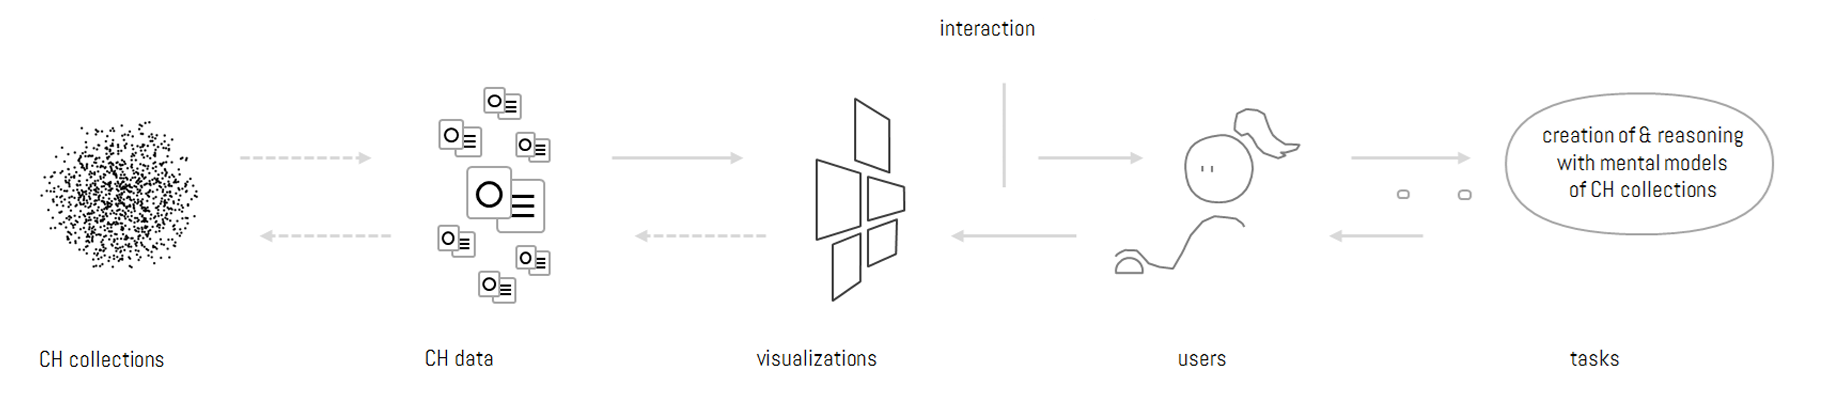
\includegraphics[width=1.0\linewidth]{ch_data}
    \caption{Schematic lineup of a of a visualization system in the CH data. ~\cite{Windhager2019Visualization}}
    \label{fig:ch_data}
\end{figure}
\FloatBarrier


The metadata can describe a broad diversity of information associated
with the \gls{CH} objects(Figure \ref{fig:ch_objects}), therefore, to classify appearances of metadata, we need to resort to a unified metadata model. 
Among several standardization initiatives, the \gls{EDM} is one of the most mature efforts. 
The \gls{EDM} reuses several existing Semantic Web vocabularies, such as the metadata set of the \gls{DCMI}, and the
\gls{CIDOC-CRM} from the \gls{CIDOC} of the International Council of Museums. 
Additionally, the target groups of digital CH collections are very diverse, from museum curators to humanities scholars and from
highly interested enthusiasts to members of the general public— \gls{CH} collections can provide useful and interesting information for all of them. 
%Consequently, many different categorizations of users exist with respect to domain expertise,
%  technical expertise, and motivation of use. There are two significant classes of users, namely experts and casual users. Experts encompass all people with a professional 
% or scientific interest in CH data, whereas casual users are lookin for personally meaningful information in everyday settings.


\begin{figure}[h!]
    \centering
    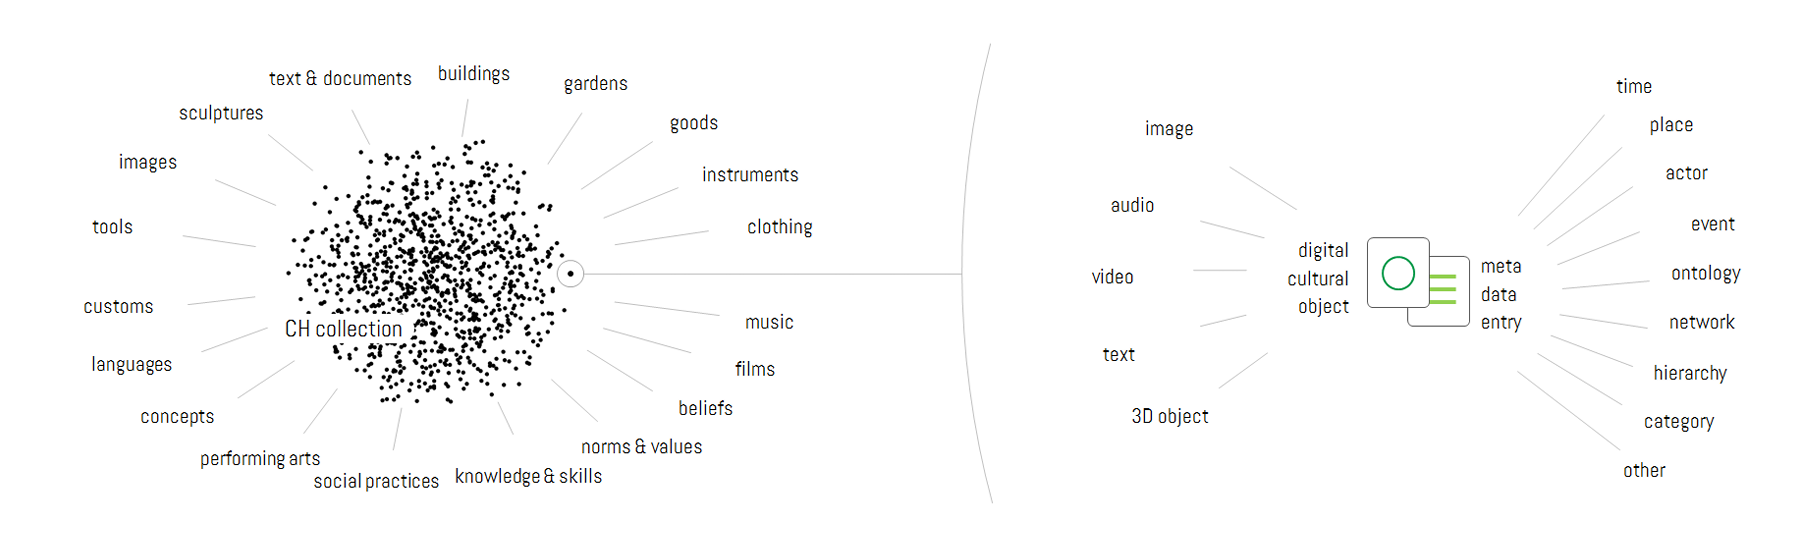
\includegraphics[width=1.0\linewidth]{metadata_entries}
    \caption{Types of cultural objects and related metadata entries. ~\cite{Windhager2019Visualization}}
    \label{fig:ch_objects}
\end{figure}
\FloatBarrier


\subsection{Virtual Heritage Environment}
\label{sec:virtual_heritage}

A \gls{VE} is a model of reality with which a human can interact, getting information 
from the model by ordinary human senses such as sight, sound, and touch and/or control
ling the model using ordinary human actions such as position and/or motion of body parts 
and voice. Usually, \gls{VE} and \gls{VR} are used synonymously, but 
some authors reserve the first one for an artificial environment that the user interacts with.  ~\cite{hale2014handbook}


Virtual heritage involves the use of computer-based interactive technologies to record, preserve, or recreate 
artifacts and sites of historical, artistic, religious, and cultural significance and to deliver 
the results openly to a global audience in such a way as to provide a formative educational 
experience through electronic manipulations of time and space. ~\cite{848434} Given the virtual objects interactivity of our project, we can derive from these definitions that we will use a \gls{VE} to represent heritage artifacts 
in \gls{3D}, enabling users to explore and interact with \gls{CH} in an immersive and educational way.

Ever since the early 1990s, there has been a worldwide interest in the prospect of using \gls{VR} to 
recreate historic sites and events for such purposes as education, special project commissions, 
and showcase features at national and World Heritage visitor centers. \gls{VR} in \gls{CH} offers a means of protecting the fragile state of some sites and can help educate visitors in how to explore, interpret, and respect them. ~\cite{hale2014handbook}




\subsection{Digital Twin}
\label{sec:digital_twin}


The \gls{DT} can be understood as a probabilistic, multiscale,
multiphysics integrated simulation of a system that uses the best physical models,
sensors, and history to mirror the life cycle of its corresponding twin. 
The \gls{DT} consists of three components: physical product in a real monitored
 space, data and information connections, and the corresponding virtual product
 in virtual space (Grieves and Vickers 2017).


 The potential application of the \gls{DT} for heritage is its realistic
 representation in the form of an intelligent and semantically enriched \gls{3D} model
\gls{HBIM}, becoming a tool capable of managing information collected and modeled,
 improving its availability and accessibility.
%  According to Nagakura et al. (2015), having a digital model of historical
%  heritage is a cheaper tool to allow building investigations because, unlike other
%  areas of study, there is no way to take buildings to laboratories or store them in
%  museums galleries like other historical artifacts.
 The use of digital scanning technologies to survey the current state of historic
 buildings, such as photogrammetry and laser scanning, expedites the process
 of generating a digital model.~\cite{dezen2020towards}

% Initially mostly applied in astronautics and aerospace area (Grieves and Vickers,
% 2016), recent progress in IoT (Internet of Things) infrastructures and the development of low-cost
% and reliable sensors has led specialists in building physics to consider such technologies to support
% monitoring strategies for the preservation of heritage sites. 
Implementing \gls{DT} for the management and preservation of \gls{CH} assets requires adopting a collaborative integrated approach and a strong
interplay among heritage recorders, conservation experts and information and communications technology specialists.
In addition to the modelling of information related to heritage sites, open standards should
be adopted for the identification of risks, damage and possible treatments to enable the awareness
of \gls{DT} with respect to their interrelationship and to ensure interoperability among the information
systems of multiple organization and institutions. Before developing preventive conservation strategies, a
good understanding of the heritage site and its context, including the assessment of its multiple values,
is necessary. In this regard, the complex management of information related to the documentation
of heritage places involves critical reflection on the adoption of an appropriate \gls{HIS}. The need for \gls{3D} visualization in \gls{GIS} to enable better
visualization and analysis of complex issues related to elements of significance has led researchers
in the field to progressively consider \gls{HBIM} as a relevant alternative.
~\cite{jouan2020digital}
%This chapter explains the key concepts related to the theme of this thesis.
% \gls


\section{Interaction and Visualization Tecnologies}
\label{sec:interaction_visualization}


\subsection{Virtual Environment Interactors}
\label{sec:interactors}


A \gls{3D} interactor is generally a geometric object with a defined behavior when certain events 
occur and certain properties of the environment and the objects in it change. 

 As is true of \gls{2D} graphical applications, a \gls{3D} environment may contain geometric objects that 
belong to a class that interact with the user and other objects in a well-defined way. In \gls{2D} interfaces, 
these objects are called widgets, components, or interactors and include buttons, menus, scrollbars, 
and pointers. Each class of object encapsulates an interactive behavior, parameterized to allow for 
multiple uses. 



\begin{figure}[h!]
    \centering
    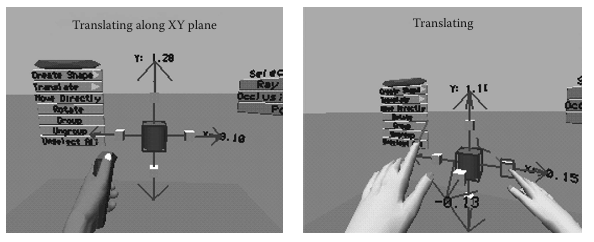
\includegraphics[width=1\linewidth]{human_interaction}
    \caption{\gls{VR} interface where a user is manipulating a \gls{3D} object. ~\cite{hale2014handbook}} %Interactors in a shape manipulation task.
    \label{fig:human_interaction}
\end{figure}
\FloatBarrier




The Figure \ref{fig:human_interaction} above contains a set of \gls{SVIFT} interactors, including buttons, menus, and tabs
that can be grabbed and moved (or bestow the grab and move ability to another object), constraint maintainers 
(e.g., keeping the manipulated object on a particular plane), and selectors. The image on the left is using a 
ray selector interactor, while the figure on the right is using a poking selector.


%CONTINUAR DAQUI
\subsection{Hardware Interaction}
\label{sec:hardware_interaction}

\subsubsection{Input Devices}
\label{sec:input_devices}
%\textbf{Input Devices}

Common \gls{VE} input devices include \gls{6-DOF} trackers\footnote{\url{https://www.ar.rocks/glossary/6dof-tracking}}, continuous posture-recognition gloves, discrete 
event gloves, pen-like devices, simple button devices, and special-purpose devices such as the 
Spaceball or force-feedback joysticks. 

Selection is simply the task of specifying an object or set of objects for some action. 
Most selection techniques can be categorized by their method of indicating of an object, whether 
done by touching it with a virtual hand, pointing at it, occluding it, encapsulating it in a volume, or 
indirectly selecting it. Manipulation goes hand in hand with selection. Manipulation refers broadly to the  modification of 
attributes of the selected object. Attributes may include position, orientation, scale, shape, color, 
or texture. For the most part, research has mainly considered the manipulation of the  position 
and orientation of rigid objects, although some special-purpose applications include object defor
mation or scaling. Object manipulation tasks have importance in such applications as design, 
prototyping, simulation, and entertainment, all of which may require environments that can be 
modified by the user. The design space for manipulation techniques is quite large. To provide a simple overview of the 
techniques already developed in the design space, three categories are presented in the following—
virtual hand, proxy, and indirect. Travel, also called viewpoint motion control, is the most ubiquitous and common \gls{VE} interaction 
task—simply the movement of the user within the environment. Travel and wayfinding make up the task of navigation. Because travel is so universal, a multitude of techniques have been proposed 
(see Mine, 1995, for a survey of early techniques). Most travel techniques can be categorized as physical locomotion, 
steering, automated, or manual manipulation. Many of the other interactions found in VE applications fall under the heading of system control. 
This category includes commands, mode changes, and other modifications of system state. 
Often, system control tasks are composites of the other universal tasks. For example, choos
ing a menu item is a selection task, whereas dragging an object to a trash can for deletion is a 
manipulation task. The categories of system control techniques include graphical 
menus, voice commands, gestures, and tools.~\cite{hale2014handbook}


\subsubsection{Output Devices}
\label{sec:output_devices}
%\textbf{Output Devices}

The three common \gls{VE} display devices are \glspl{HMD}, \glspl{SID} (fully or 
semisurrounding displays, such as the \gls{CAVE}\footnote{\url{https://steantycip.com/vr-cave/}}), and single-screen stereo displays, such as the Responsive Workbench\footnote{\url{https://graphics.stanford.edu/projects/RWB/}}. 
These display types have very different characteristics, and interaction with these displays is likely to be extremely different as well. HMDs and fully surrounding \glspl{SID} provide the ability to view the entire \gls{VE} by physically turning. Semisurrounding \glspl{SID} require the use of virtual rotations, so applications intended for such 
displays should be designed in a manner to minimize these less-desirable rotations. \glspl{HMD} that have a narrow \gls{FOV} require extensive head rotation in order for the user to see the entire environment. 



\subsection{Augmented Reality}
\label{sec:augmented_reality}

\gls{AR} aims at simplifying the user’s life by bringing virtual information not
only to his immediate surroundings, but also to any indirect view of the real-world
environment, such as live-video stream. \gls{AR} enhances the user’s perception of and
interaction with the real world. 

Computer vision renders \gls{3D} virtual objects from the same viewpoint from which the
images of the real scene are being taken by tracking cameras. Augmented reality image
registration uses different method of computer vision mostly related to video tracking.
These methods usually consist of two stages: tracking and reconstructing/recognizing. First,
fiducial markers, optical images, or interest points are detected in the camera images.
Tracking can make use of feature detection, edge detection, or other image processing
methods to interpret the camera images.

One of the most important aspects of augmented reality is to create appropriate techniques
for intuitive interaction between the user and the virtual content of \gls{AR} applications. There
are four main ways of interaction in \gls{AR} applications: tangible \gls{AR} interfaces, collaborative
\gls{AR} interfaces, hybrid \gls{AR} interfaces, and the emerging multimodal interfaces. ~\cite{carmigniani2011augmented}
Firstly, tangible interfaces support direct interaction with the real world by exploiting the use of
real, physical objects and tools. Secondly, the collaborative \gls{AR} interfaces include the use of multiple displays to support remote and colocated activities.
Following, the hybrid interfaces combine an assortment of different, but complementary interfaces as well
as the possibility to interact through a wide range of interaction devices.
Finally, multimodal interfaces combine real objects input with naturally occurring forms of language
and behaviors such as speech, touch, natural hand gestures, or gaze. This project will use an "hybrid \gls{AR} interface", which integrates various elements to create an immersive and interactive experience.
This includes the use of digital representations such as \gls{3D} models and an interactive map, alongside physical objects like the Tróia ruins and artifacts.
Additionally, the project may incorporate other input methods, such as user gestures and touch, allowing for dynamic interactions with the content. 
%By combining these diverse technologies—augmented reality (AR), digital repositories, and real-world artifacts—the project aims to provide a comprehensive platform that enhances the visitor’s experience while preserving and presenting the cultural heritage of Tróia.


\subsection{Augmented Reality vs Virtual Reality}
\label{sec:mix_reality}

While \gls{VR} technology, or \gls{VE} as called by Milgram, completely immerses users in a synthetic world
without seeing the real world, \gls{AR} technology augments the sense of reality by superimposing virtual objects and cues upon the real world in real time. 

Virtuality Continuum is defined by Paul Milgram and Fumio Kishino as a continuum that spans between the real environment
and the virtual environment comprise \gls{AR} and \gls{AV}
in between, where \gls{AR} is closer to the real world, and \gls{AV} is closer to a pure \gls{VE}, as seen in the Figure \ref{fig:mixed_reality}.

\begin{figure}[htbp]
    \centering
    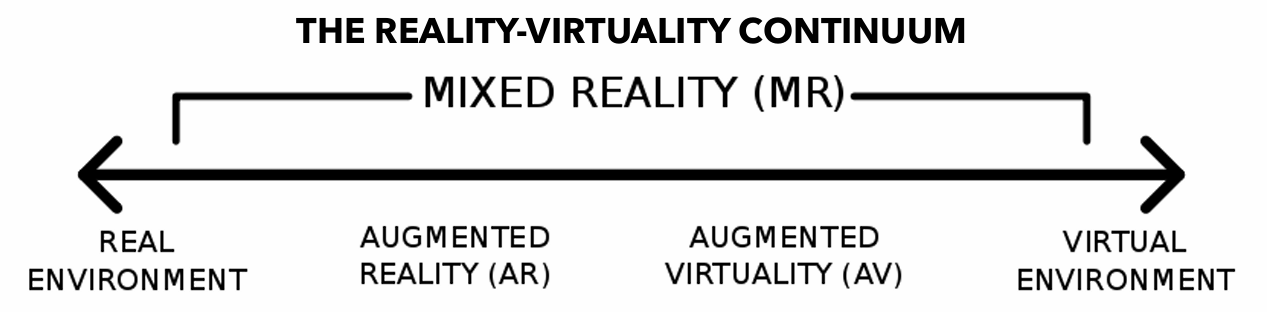
\includegraphics[width=0.8\linewidth]{mixed_reality}
    \caption{Milgram and Kishino’s Virtuality Continuum. ~\cite{milgram1994taxonomy}}
    \label{fig:mixed_reality} 
\end{figure} 
\FloatBarrier


\section{\glsentryshort{3D} Data Acquisition and Visualization}
\label{sec:data}

\subsection{Photogrammetry}
\label{sec:photogrammetry}

Photogrammetry is a measurement technique that is used to extract the geometry, displacement, and deformation of a
structure using photographs or digital images.~\cite{Baqersad2017Photogrammetry}

Concerning the object(s) of interest and the camera position(s), we distinguish
between terrestrial and aerial photogrammetry.~\cite{linder2016digital}
In aerial photogrammetry, images are acquired via overhead shots from an aircraft, providing topographic maps and land use details. In terrestrial photogrammetry, images are obtained at locations near or on the surface of
the earth and provide detailed dimensional information of an object. When the object size and the camera-to-object 
distance are both less than 100 meters, terrestrial photogrammetry is further defined as close-range photogrammetry.


Stereoscopic Viewing is a crucial photogrammetic technique to create accurate \gls{3D} models, and consists in: If we have two (or more) photos
from the same object but taken from different positions, we may easily calculate the
\gls{3D} co-ordinates of any point which is represented in both photos.~\cite{linder2016digital}

% In photogrammetry the most used model is the central projection.
%It is a geometric procedure that transforms a 3D entity into a 2D reality and it occurs when you have an object, 
%a projection centre and a projection plane oriented in any way with respect to the projected object.
%This projection is then produced because a series of straight lines (or projecting rays) connect the 
%points of the object with the projection centre and, intersecting the projection plane, generate the image points, that are the points projections.
%~\cite{aicardi2018recent}

Multi-image photogrammetry combines large groups of images to create detailed 3D models. The process begins with image acquisition, followed by importing 
the images into specialized software that automatically detects and matches correlated features. This step can be highly time-consuming and demand computer power for large datasets. 
Once matching points are identified, the software calculates their spatial relationships, producing a sparse \gls{3D} point cloud that outlines the subject’s shape, as shown in Figure \ref{fig:photo2}. 
Finally, the software refines this sparse model by reanalyzing the images to generate a much denser point cloud, similar to those produced by laser scanners.~\cite{mccarthy2014multi}

\begin{figure}[h!]
    \centering
    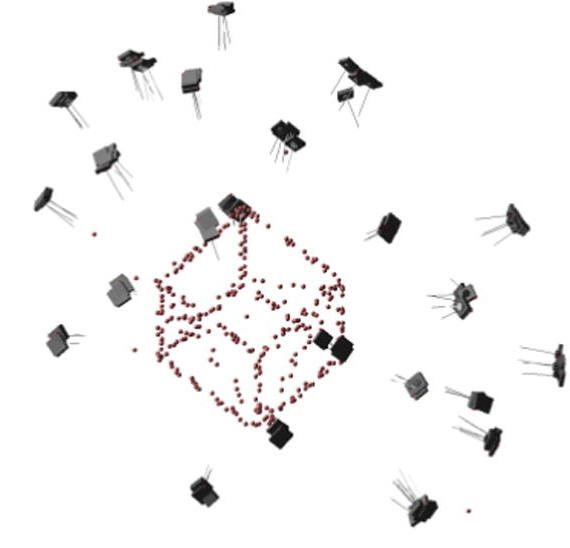
\includegraphics[width=0.45\linewidth]{photogrammetry}
    \caption{131 images of a \gls{3D} object in all-around configuration.~\cite{luhmann2016sensor}}
    \label{fig:photo2}
\end{figure} 
\FloatBarrier

 
  
The most valuable application of multi-image photogrammetry
may yet prove to be in facilitating community involvement in
archaeological recording, as well as allowing for the easy creation of
interactive \gls{3D} models which allows the public to
engage with their heritage sites in much more immersive way than
that afforded by plans and sections. In the "Previous Work", a close-range photogrammetry technique was used to generate the \gls{3D} excavation model, as detailed in section \ref{sec:photogrammetry_previous}.

\subsection{LiDAR}
\label{sec:lidar}

\gls{LiDAR} sensors enable  enable precise 3D sensing of objects and are widely used in metrology, environment monitoring, archaeology, and robotics.
This technology allows for accurate determination of an object’s distance and velocity. 
Similar to photogrammetry, \gls{LiDAR} scanning is classified into two main types: terrestrial and airborne.
The three most significant approaches in \gls{LiDAR} technology are mechanical, nanophotonics-based, and solid-state.
In traditional \gls{LiDAR} sensors, as shown in Figure \ref{fig:mechanical_LIDAR}, a mechanical rotator is used for optical beam scanning, which introduces limitations on their reliability, size, and cost.~\cite{li2022progress}

 
\begin{figure}[h!]
    \centering
    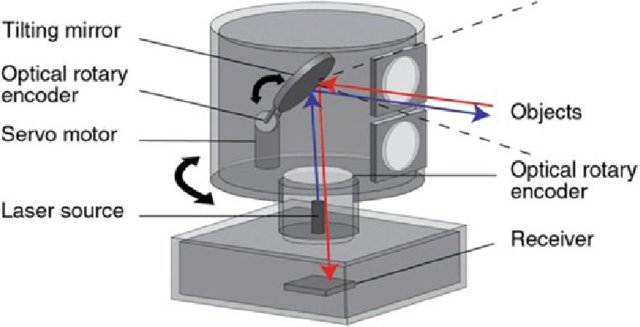
\includegraphics[width=0.6\linewidth]{mechanical_LIDAR}
    \caption{Mechanical Spinning \gls{LiDAR}.~\cite{inbook}}
    \label{fig:mechanical_LIDAR}
\end{figure} 
\FloatBarrier


Solid-state \gls{LiDAR} presents an alternative to traditional \gls{LiDAR} by eliminating the need for a bulky mechanical rotator. %, visualization example in Figure \ref{fig:flash_based}.
Moreover, advancements in optical technology have led to the development of nanophotonics-based devices with high potential and superior advantages for \gls{LiDAR} sensors. %An example of its usage in Figure \ref{fig:sequential_ilumination}. 
Different scanning techniques produce diverse types of scan outputs. For instance, flash-based LiDAR from solid-state approach captures a full-frame \gls{3D} image in a single snapshot, as shown in Figure \ref{fig:flash_based}, while sequential illumination-based LiDAR scans objects by sequentially illuminating small regions, producing the whole frame, as depicted in Figure \ref{fig:sequential_ilumination}.

\begin{figure}[h!]
    \centering
    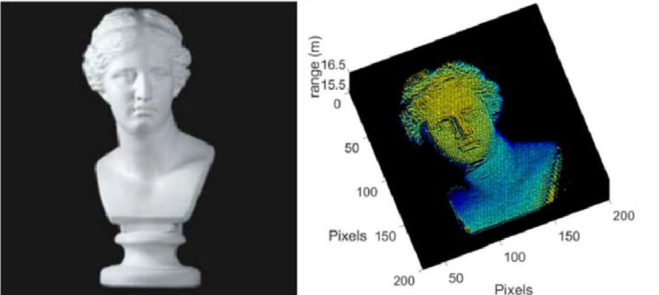
\includegraphics[width=0.65\linewidth]{flash_based}
    \caption{Flash-based \gls{LiDAR} sensor. \small{Left: \gls{2D} image of sensing target, Right: Captured \gls{3D} image.} ~\cite{li2022progress}}
    \label{fig:flash_based}
\end{figure} 



\begin{figure}[h!]
    \centering
    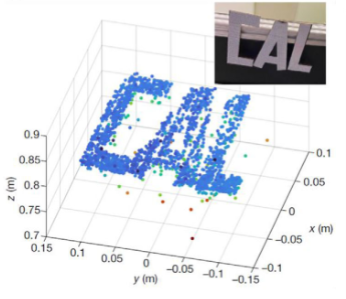
\includegraphics[width=0.45\linewidth]{sequential_ilumination}
    \caption{A \gls{LiDAR} sensor based on sequential illumination.~\cite{li2022progress}}
    \label{fig:sequential_ilumination}
\end{figure} 

\FloatBarrier

\subsection{Artifacts Reconstruction}
\label{sec:reconstruction}

Systems capable of automatically reconstructing objects from their fragments can greatly aid in the study of many civilizations.
Automated reconstruction systems working from large databases of digitized fragments could uncover numerous partial or
complete reconstructions of artifacts that may have been excavated during different years of the same excavation, or possibly
from different sites altogether. In this way, reconstruction systems not only save researchers time but, given a sufficient data
base of fragments, also have the capacity to reconstruct artifacts that would have otherwise remained as an incoherent pile of disjoint fragments.
~\cite{willis2008computational}

A precise shape measurement can be achieved using advanced laser scanners or other commercially available shape measuing devices based on stereo 
vision or structured light. A detailed triangulated \gls{3D} model of a corrupted shape is the prerequisite for its subsequent reconstruction. 
Missing or scarred parts of a shape can be reconstructed only by exploiting information from similar parts either from the same
object or on some other object. In the former case we can often utilize shape symmetries such as symmetrical parts on
human or animal bodies. Scarred parts are removed using the surface spline patches.~\cite{7801178}



\section{\gls{GIS}}
\label{sec:geographic_information_system}

A \gls{GIS} is a computer system for capturing, storing, checking, and displaying data related to positions on Earth’s 
surface. By relating seemingly unrelated data, GISs can help individuals and organizations better understand spatial patterns and relationships.
~\cite{natgeo_2024}

In \gls{GIS} there are several key iniciatives, two of the most significant are the \gls{OGC}\footnote{\url{https://www.ogc.org/}} and the \gls{OSGeo}\footnote{\url{https://www.osgeo.org/}}.  
The \gls{OGC} is an international voluntary consensus standards organization, constituting more than 450 strong—united organizations(such as Esri, Nasa), they develop open standards that ensure interoperability between diverse \gls{GIS}.~\cite{ogc_who_we_are, ogcapi}
The \gls{OSGeo} is an organization that promotes global adoption of open geospatial technology through an open philosophy and community driven development.~\cite{osgeo_about}

\subsection{Geospatial Data} 
\label{sub:geospatial_data}

\gls{GIS} applications may include diverse spatial data types, such as cartographic data, photographic data, digital data, or data in spreadsheets. Once all the desired data have been entered into a \gls{GIS} system, 
they can be combined to produce a wide variety of individual maps, depending on which data layers are included. 
One of the most common uses of \gls{GIS} technology involves comparing natural features with human activity, as illustrated in the Figure \ref{fig:gis} below. 


\begin{figure}[h!]
    \centering
    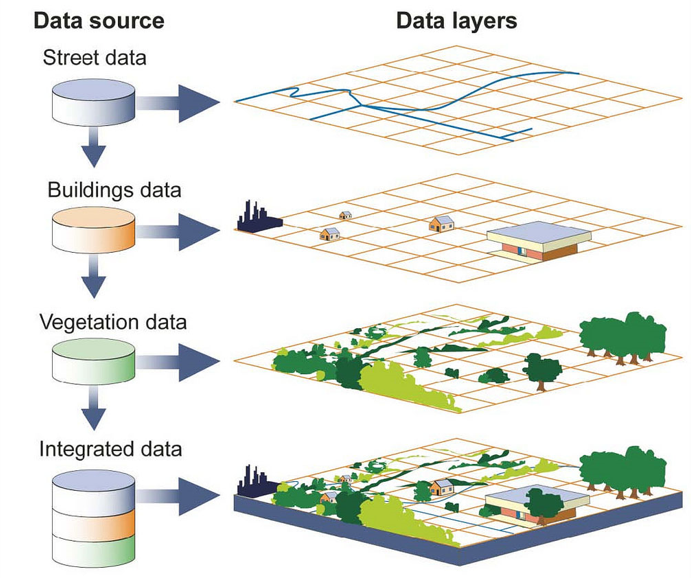
\includegraphics[width=0.6\linewidth]{gis}
    \caption{Visual representation of data layers integration in \gls{GIS}. ~\cite{gao_data_layers}}
    \label{fig:gis}
\end{figure}
\FloatBarrier

\subsection{GIS Applications in Archaeology}
\label{sub:gis_archeology}

The application of \gls{GIS} in archaeology has brought about a transformative shift, equipping archaeologists with powerful tools to gather, analyze, 
and visualize geospatial data from archaeological sites. Since 2000, archaeologists began employing \gls{GIS} for more complex spatial analyses, including landscape analysis and site distribution 
patterns. Additionally, the development of \gls{3D} \gls{GIS} technology enabled archaeologists to reconstruct ancient sites in virtual environments, offering a 
better understanding and visualization of archaeological site structures and layouts. ~\cite{yao2023overview}


\gls{GIS} serves as an invaluable platform for the comprehensive management of \gls{CH} resources. It excels in handling a wide array of
unstructured data related to \gls{CH}, allowing for a more organized and efficient approach to preservation efforts. One significant 
application of \gls{GIS} is in the inventorying of \gls{CH} sites. This encompasses a diverse range of sites, from archaeological to 
architectural and historical structures. Traditional recording methods often face limitations in terms of speed and accuracy when
it comes to gathering and assessing current situation data. Moreover, these methods may not be well-suited for conducting quantitative 
scientific management and in-depth analysis. 

In tandem with the advent and maturation of technologies like \gls{3D} computer graphics, high-resolution rendering, artificial intelligence, 
and \gls{3D} printing, these advanced methodologies have progressively found widespread application in the cultural relic preservation, 
augmenting endeavors in the preventive protection and restoration of cultural artifacts. In archaeological research, one of the most fundamental applications of GIS lies in managing spatial data dedicated on archaeological sites.
\glspl{GIS} often incorporate spatial databases, such as PostgreSQL/PostGIS or Oracle Spatial, to store and query spatial information efficiently. 
Moreover, specialized computer software, such as ArcGIS Pro or QGIS is used to visualize, analyze, and interpret this data. These \glspl{GIS} process archaeological data in 
accordance with specific data standards and protocols.

\section{Standarts and Documentation} 
\label{sub:standart}

Standards are critical for systematic and robust development of any emerging technology. 
Specification standards provide for practical descriptions of product characteristics and limitations, 
critical to an end user. Interface standards allow for interchangeability of components developed by 
different manufacturers, thus permitting specialization and robust competition in the marketplace. 
Safety standards ensure the health and safety of product users. Finally, terminology standards ensure that 
technical terminology is used in a consistent and rigorous manner, thus preventing confusion and 
ambiguity in scientific and technical reports and specifications.
~\cite{hale2014handbook}

International standards and ontologies for data encoding are crucial
to speed up interoperability and the process of integration. \gls{CIDOC-CRM}, which is created to capture the richness typical of CH
information, fully fits our needs: its classes and properties
work perfectly to capture the concepts underlying database structures, providing a high level of data integration.
~\cite{eide2008encoding}



\subsection{\glsentryshort{CIDOC} Conceptual Reference Model} 
\label{sec:cidoc}


The \gls{CIDOC-CRM}\footnote{\url{https://cidoc-crm.org/}} is a theoretical and practical tool for integrating \gls{CH} information. It provides formal definitions and a structured framework to describe concepts and relationships that support the organization and connection of information regarding \gls{CH} objects and their contexts(Figure \ref{fig:cidoc}).
Since 2006, CIDOC CRM has been recognized as an official ISO standard (\texttt{ISO 21127:2023}). The most recent version establishes \gls{CIDOC-CRM} as a compatible interface for \gls{OGC} standards, enhancing its application in \gls{GIS} and facilitating geospatial and spatiotemporal reasoning.


\begin{figure}[h!]
    \centering
    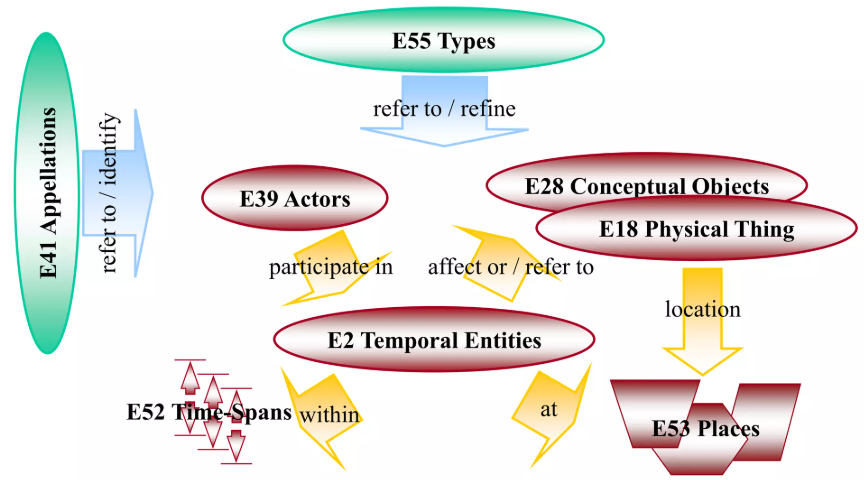
\includegraphics[width=0.7\linewidth]{CIDOC_ISO21127}
    \caption{Fundamental concepts of \texttt{ISO 21127} ~\cite{doerr2007cidoc}}
    \label{fig:cidoc}
\end{figure}
\FloatBarrier

\noindent \textbf{From database to \gls{CIDOC-CRM}} \\
The necessary information is extracted from different archaeological and museum collection data models (with various structured, as well as non-structured
data, i.e. text description) to a common standard based on \gls{CIDOC-CRM} compliant structure.
~\cite{eide2008encoding}




\section{Cultural Heritage Cloud}
\label{sec:ch_cloud}

The \gls{ECCCH}\footnote{\url{https://www.echoes-eccch.eu/}} is a European Union initiative 
to create a shared digital infrastructure that connects \gls{CH} institutions and professionals across the \gls{EU}.
The \gls{ECCCH} aims to add a digital dimension to \gls{CH} preservation, conservation, restoration, and enhancement 
by providing cutting-edge technology for artefact digitisation and artwork research. 
In Portugal, the \gls{ICOM}\footnote{\url{https://icom-portugal.org/}} is a beneficiary of the initiative, while \gls{CRUSOE}\footnote{\url{https://redcrusoe.com/}} is an \gls{ECCCH} association partner. \gls{CRUSOE} is a university association comprising institutions from both Portugal and Spain.
While \gls{ICOM} Portugal and \gls{CRUSOE} represent the participants in Portugal, the \gls{ECCCH} also includes other 14 countries' beneficiaries, affiliated entities and/or associated partners across Europe that actively support those \gls{CH} sectors enumerated above.~\cite{ecchoes}


\begin{figure}[h!]
    \centering
    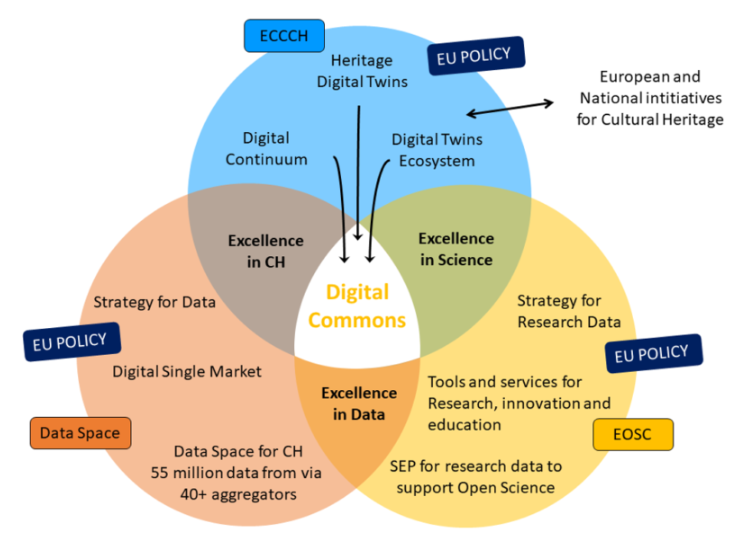
\includegraphics[width=0.7\linewidth]{echoes}
    \caption{\gls{ECHOES} goals. ~\cite{ecchoes}} 
    \label{fig:echoes}
\end{figure}
\FloatBarrier


%----------------------------------------------------------------------
	  %   \midrule
	  % \classoption{linkscolor}%
	  %   {A color of your choice.}%
	  %   {The color for all the hyperlinks in the PDF file.}%
	  %   {\defaultopt{darkblue}
	  %    The “\texttt{media=paper}” option (see below) will override this option to “\texttt{black}”}
% %----------------------------------------------------------------------
%     \midrule
%   \classoption{media}%
%     {screen, paper}%
%     {The target of the PDF.}%
%     {\defaultopt{screen}
%      By default, PDF for screen has colored links and identical left and right margins, while PDF for paper (to print) has black links and may have different left and right margins.}
%     \midrule
% %----------------------------------------------------------------------
%   \classoption{print/index}%
%     {true, false}%
%     {Produce the document index.}%
%     {\defaultopt{false}
%      The index (\emph{índice remissivo}) is a keyword index typeset an the end of the document. WARNING: Should not be confused with the table of contents.}
%     \midrule
%
%
%
%
% %----------------------------------------------------------------------
%   \classoption{fontstyle}%
%     {bookman, charter, fourier, kpfonts(*), mathpazo1, mathpazo2, newcent}%
%     {The font set to be used in the document.}{Please note that a font set include definitions for the main text, headings, maths, etc.}
%     \midrule
% %----------------------------------------------------------------------
%   \classoption{chapstyle}%
%     {bianchi, bluebox, brotherton, dash, default, elegant(*), ell, ger, hansen, ist, jenor, lyhne, madsen, pedersen, veelo, vz14, vz34, vz43}%
%     {The chapter style}{The look of the chapter beginning.}
%     \midrule
% %----------------------------------------------------------------------
%   \classoption{converlang}%
%     {en, pt(*)}%
%     {The language to be used when typesetting the cover page.}{}
%     \midrule
% %----------------------------------------------------------------------
%   \classoption{otherlistsat}%
%     {front(*), back}%
%     {Where to put the other lists besides the table of contents.}{The default is (\texttt{front}) before the main text.  But some scientific areas prefer them at the end of the document (\texttt{back}), just before the Appendixes.}
%     \midrule
% %----------------------------------------------------------------------
%   \classoption{statement}%
%     {true, false(*)}%
%     {Include or don't include the contents of the “\texttt{statement}” file.}{The default is for this file to be ignored (if it exists).}
%     \midrule
% %----------------------------------------------------------------------
%   \classoption{spine}%
%     {true, false(*)}%
%     {Generate the book spine and the last page in the PDF.}{}
%     \midrule
% %----------------------------------------------------------------------
%   \classoption{biblatex}%
%     {OPT=\{list of options for \texttt{biblatex}\}}%
%     {Customize \texttt{biblatex}, the bibliography management system used in this class.}{Probably you will want to change the value of the \texttt{biblatex} “\texttt{style}” option. For other customizations of \texttt{biblatex} check its manual.}
%     \midrule
% %----------------------------------------------------------------------
%   \classoption{memoir}%
%     {OPT=\{list of options for \texttt{memoir}\}}%
%     {Customize the base class \texttt{memoir}.}{The \texttt{memoir} manual should be the first document to be consulted when looking for “\textbf{how can I do this?}” You may what to change the base font size from 11pt to a smaller (10pt) or larger (12pt) size.  Also, remember to change the “\texttt{draft}” to final when your document is finished.}
%     \midrule
   % \bottomrule
%\end{xltabular}
%\egroup
% \end{ctabular}



% \todo[inline]{A a note in a line by itself.}
%

% Reference to Potassium \gls{chem:potassio} and Sodium \gls{chem:sodio} as well.

%
% Please note that
% \begin{center}
%   \textbf{\large this package and template are not official for FCT/NOVA}.
% \end{center}



% \printbibliography[heading=subbibliography, segment=\therefsegment, title={\bibname\ for chapter~\thechapter}]



% section folder_structure (end)

% ===================
% = Package options =
% ===================




% \printbibliography[heading=subbibliography, segment=\therefsegment, title={\bibname\ for chapter~\thechapter}]